\documentclass{article}
\usepackage[utf8]{inputenc}
\usepackage{graphicx}
\usepackage[table,xcdraw]{xcolor}
\usepackage{float}
\usepackage{amsmath}
\usepackage{amssymb}
\usepackage{hyperref}
\usepackage{pdfpages}
\usepackage{polski}
\usepackage{longtable}
\usepackage{bm}
\begin{document}

\begin{titlepage}
   \begin{center}
   
       \textbf{\huge Wykorzystanie poznanych metod dotyczących analizy zależności liniowej do wybranych danych rzeczywistych}

       \vspace{1cm}
            
       \textbf{\Large Autorzy}\\
       \vspace{0.5cm}
       Mateusz Stasiak 262339\\
       Karolina Wypych 262333\\
            
       \vspace{1cm}
     
       
\includegraphics[width=0.7\textwidth]{images/logo_pwr.png}
       
       \vspace{0.8cm}
       Wydział Matematyki\\
       24 grudnia 2022r.
            
   \end{center}
\end{titlepage}
\tableofcontents
\newpage
\section{Wprowadzenie}
W analizie danych przeważnie ma się do czynienia z dużymi zbiorami. Wybór odpowiednich metod do ich przetwarzania jest kluczowy. Zdarza się, że po przedstawieniu zmiennych na wykresie punktowym, można dostrzec, że w przybliżeniu układają się w linii prostej. Wówczas pod pewnymi warunkami, jest to dobry moment na zastosowanie metody regresji liniowej. 
Te warunki to:
\begin{itemize}
    \item Zmienne powinny mieć charakter ciągły. 
    \item Obserwacje powinny być od siebie niezależne (tzn. nie mogą występować żadne zależności).
    \item W danych nie powinny występować żadne istotne elementy odstające. 
    \item Błedy (residua, wartości resztkowe) linii najlepszego dopasowania powinny mieć rozkład normalny.
    \end{itemize}
Celem niniejszego raportu jest sprawdzanie tych warunków i próba przewidzenia cen domów w zależności od średnich przychodów w ich okolicy. Wszystkie analizy przeprowadzone zostały za pomocą języka Python i jego bibliotek.
\section{Dane}
Dane użyte w raporcie zostały pobrane ze strony \href{https://bit.ly/3YOdcKU}{nickmccullum.com}. Zawierają informacje na temat m.in. przeciętnych przychodów i liczby pokoi w okolicy danego domu, ceny sprzedaży i adresu.

\subsection{Wczytanie i przygotowanie danych}
Dane zostały wczytane z pliku .csv za pomocą funkcji \texttt{pd.read\_csv()}. Nastęnie wybrano dwie kolumny - opisujące przeciętny dochód oraz cenę domu, które są zmiennymi ciągłymi, a poszczególne obserwacje są od siebie niezależne (np. cena domu w jednej części kraju nie zależy od ceny w innej). Na ich podstawie zostaną przeprowadzone wszystkie dalsze analizy mające na celu przewidzenie cen mieszkań.
W rozważanym modelu zmienną niezależną będzie przeciętny dochód a zależną cena domu. 

\begin{table}[H]
\centering
\resizebox{\textwidth}{!}{%
\begin{tabular}{|l|l|l|l|l|}
\hline
\rowcolor[HTML]{F2B7D6} 
\textbf{nazwa zmiennej}                          & \textbf{status}    & \textbf{opis zmiennej}                                                                                & \textbf{rodzaj zmiennej} & \textbf{typ zmiennej} \\ \hline
\multicolumn{1}{|c|}{\textbf{przeciętny dochód}} & zmienna zależna    & \begin{tabular}[c]{@{}l@{}}przeciętny dochód osób zamieszkujących \\ okolice danego domu\end{tabular} & ciągła                   & float                 \\ \hline
\textbf{cena domu}                               & zmienna niezależna & kwota za jaką sprzedano dany dom                                                                      & ciągła                   & float                 \\ \hline
\end{tabular}%
}
\caption{Charakterystyka zmiennych}
\label{zmienne}
\end{table}
\section{Analiza jednowymiarowa zmiennych}
Przed przystąpieniem do budowania modelu regresji liniowej należy przyjrzeć się każdej zmiennej z osobna. Pozwala to w łatwy sposób wychwycić obserwacje odstające i najczęściej przyjmowane wartości.

\subsection{Zmienna niezależna}

W pierwszej kolejności rozważaniom poddano ceny domów, będące zmienną niezależną. Zwizualizowano je na wykresach, a także obliczono podstawowe miary miary położenia, rozproszenia, skośności i spłaszczenia.

\subsubsection{Wizualizacja danych} \label{wizual_zależna}

Wizualizacja danych jest niezwykle istotna przy ich analizowaniu. By lepiej poznać rozważaną zmienną, warto wykonać kilka wykresów. Ułatwią one zidentyfikowanie najczęściej pojawiających się wartości oraz rozkładu, z którego pochodzą dane.\\\\
Jako pierwszy wygenerowano wykres pudełkowy i to od niego rozpoczęto analizę obserwacji.
    \begin{figure}[H]
	\begin{center}
		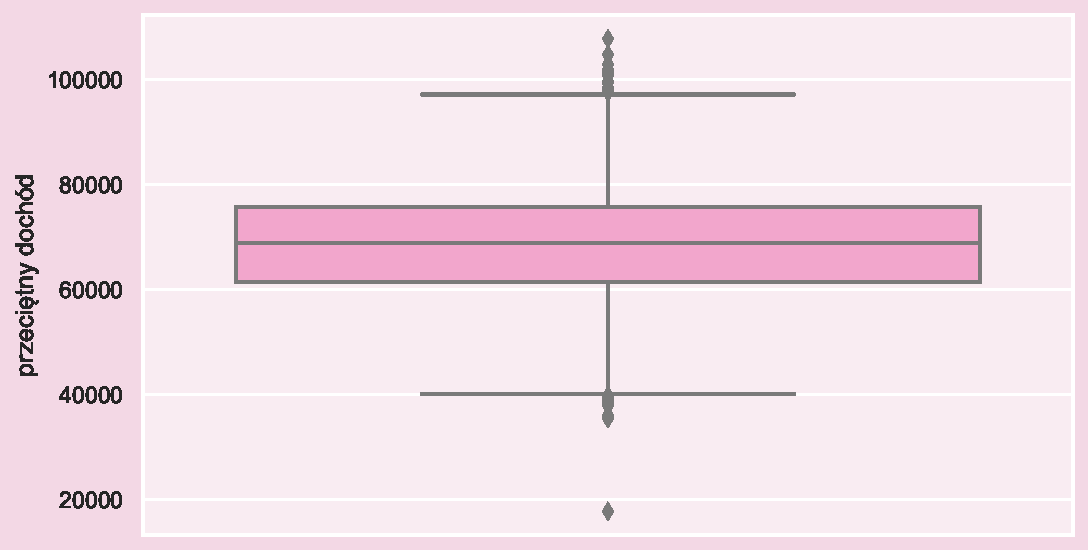
\includegraphics[scale=0.68]{images/income_box.pdf}
		\caption{Wykres pudełkowy przeciętnych przychodów}
		\label{fig:income_box}
	\end{center}
	\end{figure}
\noindent Powyższy wykres dostarcza kilku istotnych informacji. $50\%$ wszystkich obserwacji znajduje się wewnątrz pudełka, a przecinająca je pionowa linia jest medianą rozważanego zbioru danych, która dzieli go na połowy. Stąd widać, że ponad połowa osób zarabia między $60 000$ a $80 000$. Wąsy natomiast łączą pudełko z największą i najmniejszą wartością badanej zmiennej odpowiednio z przedziału $(Q1 - 1,5 \cdot IQR; Q1)$ oraz $(Q3;Q3 + 1,5 \cdot IQR)$. Zatem w pierwszym z nich mieści się $25\%$ obserwacji o wartościach niższych od dolnego kwartyla a w drugim wyższych od górnego. Pozwala to wywnioskować, że zdecydowana większość społeczeństwa zarabia od $40 000$ do niemal $100000$. Na wykresie nie brak także wartości odstających, które oznaczają zarobki znacznie odbiegające od reszty. 

   
 \noindent Można także spróbować wyznaczyć rozklad z jakiego pochodzą omawiane obserwacje. W tym celu należy narysować jej dystrybuantę empiryczną i wykorzystać fakt, że dystrybuanta jednoznacznie określa rozkład.
    \begin{figure}[H]
	\begin{center}
		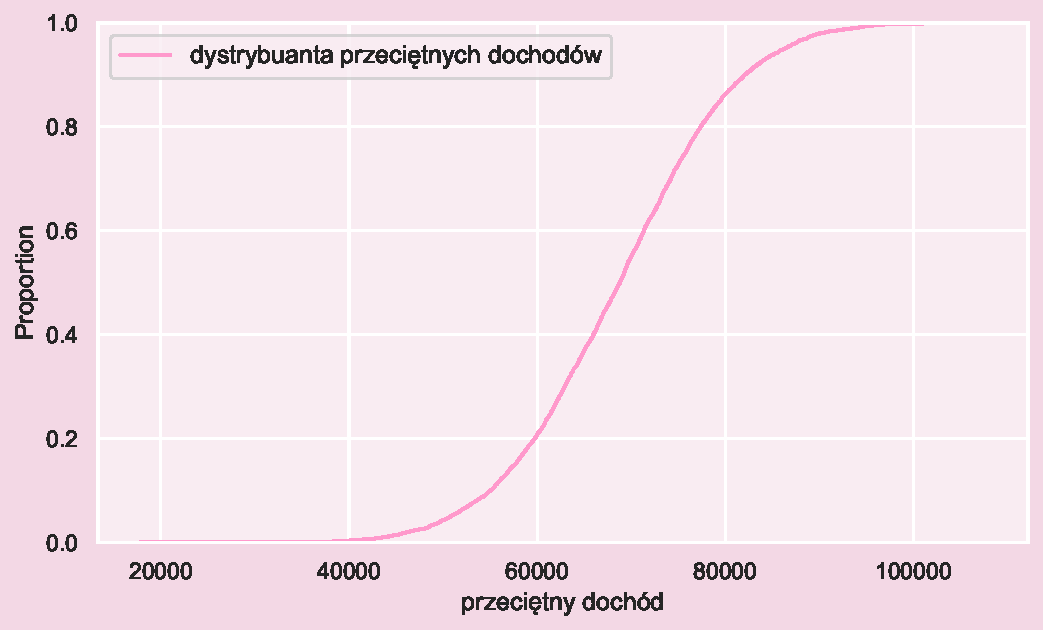
\includegraphics[scale=0.68]{images/income_dystr1.pdf}
		\caption{Dystrybuanta empiryczna przeciętnych przychodów.}
		\label{denistyx}
	\end{center}
	\end{figure}
\noindent Wykres kształtem przypomina rozkład normalny, dlatego bardzo prawdopodobne wydaje się, że szukanym rozkładem będzie właśnie ten rozkład. By potwierdzić lub odrzucić tę tezę obliczono średnią i wariancję danych, które wyniosły kolejno $\mu \approx 68583 $, $\sigma^2 \approx 113570058$, a następnie dorysowano dystrybuantę teoretyczną $\mathcal{N}$$(\mu,\sigma^2)$.

    \begin{figure}[H]
	\begin{center}
		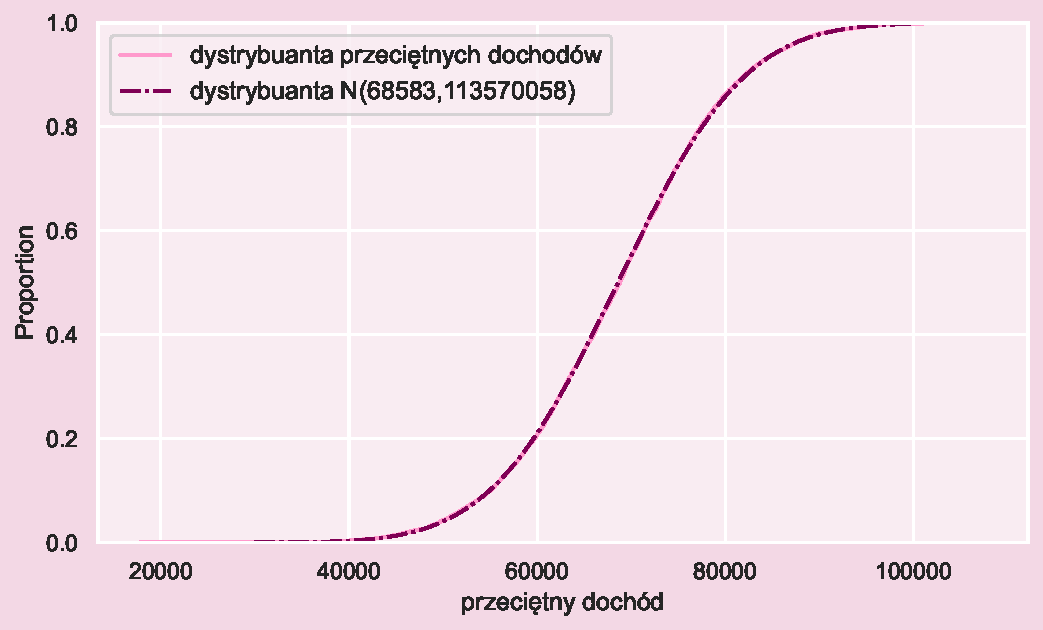
\includegraphics[scale=0.68]{images/income_dystr.pdf}
		\caption{Zestawienie dystrybuanty empirycznej i teoretycznej}
		\label{fig:income_dystr}
	\end{center}
	\end{figure}

\noindent Z wykresu \ref{fig:income_dystr}. widać, że obie dystrybuanty pokrywają się ze sobą na całej długości, co świadczy o tym, że rozkład i jego parametry zostały prawidłowo dobrane. Na pierwszy rzut oka tak duże wartości mogą się wydawać podejrzane, jednak patrząc na to, że rozpatrywane obserwacje przekraczają nawet $100 000$ trzeba przyznać, że są one prawidłowe.\\\\

\noindent Ostatnim etapem wizualizacji zmiennej niezależnej jest narysowanie histogramu prawdopodobieństwa i gęstości empirycznej.

    \begin{figure}[H]
	\begin{center}
		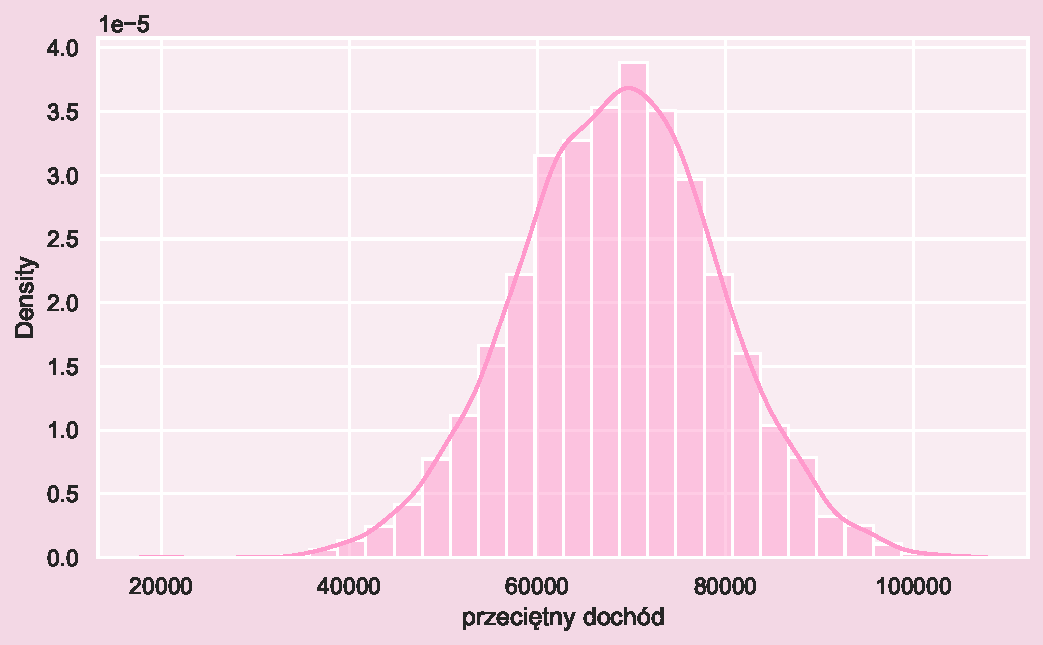
\includegraphics[scale=0.68]{images/income_hist.pdf}
		\caption{Histogram przeciętnych dochodów wraz z gęstością empiryczną.}
		\label{denistyx}
	\end{center}
	\end{figure}

 \noindent Wykres ten potwierdza informacje, które wyczytano z boxplotu na wykresie \ref{fig:income_box}. Osoby zarabiające około $70000$ stanowią najliczniejszą grupę. Większość skupiona jest pomiędzy $50000$ i $90000$, a najniższe słupki odnotowuje się poniżej $20000$ i powyżej $100 000$. Histogram i dorysowana gęstość empiryczna swoim kształem jedynie potwierdzają wyznaczony wcześniej rozkład normalny. Dla pewności dorysowano jednak gęstość teoretyczną o wyliczonych wcześniej parametrach, która ponownie pokryła wykres empiryczny.
 
    \begin{figure}[H]
	\begin{center}
		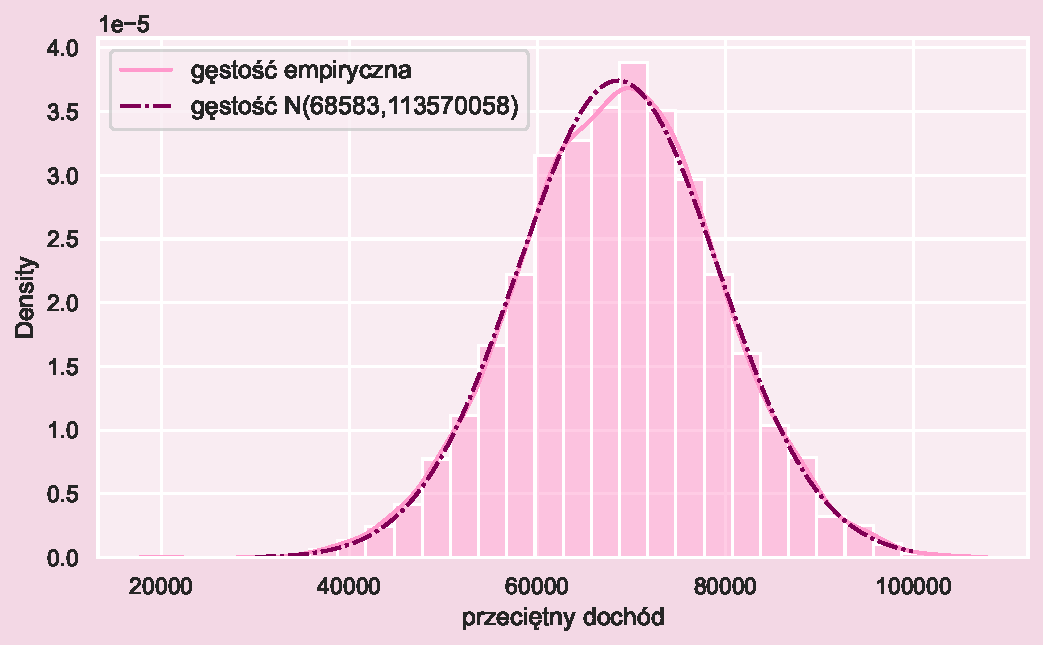
\includegraphics[scale=0.68]{images/income_hist_teor.pdf}
		\caption{Histogram przeciętnych dochodów wraz z empiryczną i teoretyczną gęstością.}
		\label{denistyx}
	\end{center}
	\end{figure}
 
\subsubsection{Podstawowe miary}
Dodatkowych informacji o danych dostarcza także obliczenie podstawowych miar. Dla zwiększenia przejrzystości wyniki zaprezentowano w tabeli. 

\begin{table}[H]
\centering
\resizebox{\textwidth}{!}{%
\begin{tabular}{|cccccc|}
\hline
\rowcolor[HTML]{F66BB4} 
\multicolumn{6}{|c|}{\cellcolor[HTML]{F66BB4}\textbf{miary rozproszenia}}                                                                                                                                                                                                                                                                        \\ \hline
\rowcolor[HTML]{F2B7D6} 
\multicolumn{1}{|c|}{\cellcolor[HTML]{F2B7D6}\textbf{Q1}}  & \multicolumn{1}{c|}{\cellcolor[HTML]{F2B7D6}\textbf{Q3}}  & \multicolumn{1}{c|}{\cellcolor[HTML]{F2B7D6}\textbf{IQR}}      & \multicolumn{1}{c|}{\cellcolor[HTML]{F2B7D6}\textbf{wariancja}} & \multicolumn{1}{c|}{\cellcolor[HTML]{F2B7D6}\textbf{std}} & \textbf{wsp. zmienności} \\ \hline
\rowcolor[HTML]{F5F5F5} 
\multicolumn{1}{|c|}{\cellcolor[HTML]{F5F5F5}61480.562388} & \multicolumn{1}{c|}{\cellcolor[HTML]{F5F5F5}7.578334e+04} & \multicolumn{1}{c|}{\cellcolor[HTML]{F5F5F5}14302.776278}      & \multicolumn{1}{c|}{\cellcolor[HTML]{F5F5F5}1.135701e+08}       & \multicolumn{1}{c|}{\cellcolor[HTML]{F5F5F5}10656.925361} & 15.540257                \\ \hline
\multicolumn{6}{|l|}{}                                                                                                                                                                                                                                                                                                                           \\ \hline
\rowcolor[HTML]{F66BB4} 
\multicolumn{6}{|c|}{\cellcolor[HTML]{F66BB4}\textbf{miary położenia}}                                                                                                                                                                                                                                                                           \\ \hline
\rowcolor[HTML]{F2B7D6} 
\multicolumn{2}{|c|}{\cellcolor[HTML]{F2B7D6}\textbf{śr. arytm.}}                                                      & \multicolumn{1}{c|}{\cellcolor[HTML]{F2B7D6}\textbf{śr.harm.}} & \multicolumn{1}{c|}{\cellcolor[HTML]{F2B7D6}\textbf{śr. geom.}} & \multicolumn{2}{c|}{\cellcolor[HTML]{F2B7D6}\textbf{mediana}}                        \\ \hline
\rowcolor[HTML]{FFFFFF} 
\multicolumn{2}{|c|}{\cellcolor[HTML]{FFFFFF}6.858311e+04}                                                             & \multicolumn{1}{c|}{\cellcolor[HTML]{FFFFFF}6.681637e+04}      & \multicolumn{1}{c|}{\cellcolor[HTML]{FFFFFF}6.772310e+04}       & \multicolumn{2}{c|}{\cellcolor[HTML]{FFFFFF}6.880429e+04}                            \\ \hline
\rowcolor[HTML]{FFFFFF} 
\multicolumn{6}{|l|}{\cellcolor[HTML]{FFFFFF}}                                                                                                                                                                                                                                                                                                   \\ \hline
\rowcolor[HTML]{F66BB4} 
\multicolumn{6}{|c|}{\cellcolor[HTML]{F66BB4}{\color[HTML]{000000} \textbf{miary skośności i spłaszczenia}}}                                                                                                                                                                                                                                     \\ \hline
\rowcolor[HTML]{F2B7D6} 
\multicolumn{3}{|c|}{\cellcolor[HTML]{F2B7D6}wsp. skośności}                                                                                                                            & \multicolumn{3}{c|}{\cellcolor[HTML]{F2B7D6}kurtoza}                                                                                                   \\ \hline
\rowcolor[HTML]{FFFFFF} 
\multicolumn{3}{|c|}{\cellcolor[HTML]{FFFFFF}-0.033710}                                                                                                                                 & \multicolumn{3}{c|}{\cellcolor[HTML]{FFFFFF}0.044329}                                                                                                  \\ \hline
\end{tabular}%
}
\caption{Miary dla przeciętnych przychodów}
\label{miary_income}
\end{table}


\noindent Część z przedstawionych miar została już omówiona w paragrafie \ref{wizual_zależna}, ale to na co należy szczególnie zwrócic uwagę to wartość kurtozy. Ponieważ biblioteka \textit{scipy} w Pythonie przyjmuje za kurtozę rozkładu normalnego $0$, otrzymana $K = 0.044329$ stanowi kolejne potwierdzenie prawidłowego wyznaczenia rozkładu zmiennej. 

\subsubsection{Wnioski}
Podsumowując cały rozdział poświęcony  zmiennej zależnej można stwierdzić, że zrealizowano pierwsze cele raportu. Wnikliwe przeanalizowanie zmiennej za pomocą wykresów i miar rozproszenia pozwoliło zobaczyć jak rozmieszczone są dane i zidentyfikowac ich rozkład jako $\mathcal{N}$$(\mu,\sigma^2)$.  Ponadto pokazano, że nie zawierają żadnych istonie odstających wartości, co czyni je dobrą podstawą budowy modelu regresji liniowej.

\subsection{Zmienna zależna}
W drugiej kolejności przeanalizowano ceny domów, będące zmienną niezależną. Podobnie jak dla przeciętnych dochodów zwizualizowano je na wykresach i obliczono podstawowe miary. 

\subsubsection{Wizualizacja danych}
Poprzedni podrozdział udowodnił, jak potężnym narzędziem jest wizualizacja danych i ilu informacji można doszukać się poprzez wygenerowanie zaledwie kilku wykresów. Dlatego przy analizowaniu zmiennej zależnej nie sposób pominąć tego kroku.
Najpierw wygenerowano boxplot, z którego odczytano, że najpopularniejsze ceny mieszkań mieszczą się w przedziale $1-1.5$ miliona. Tym razem ponownie nie brakuje wartości odbiegających od pozostałych. Z wykresu można odczytać, że są to wartości, które przekroczyły około $2.2$ miliona lub nie dosięgnęły $300$ tysięcy.
    \begin{figure}[H] 
	\begin{center}
		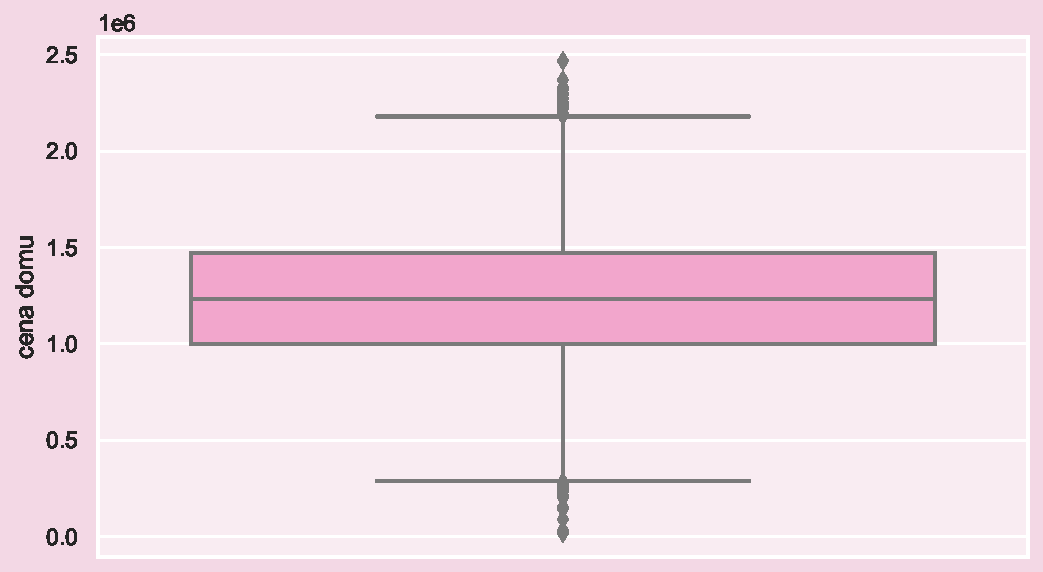
\includegraphics[scale=0.68]{images/price_box.pdf}
		\caption{Wykres pudełkowy cen domów}
		\label{denistyx}
	\end{center}
	\end{figure}
 
\noindent Następnie narysowano dystrybuantę empiryczną, która tym razem ponownie bardzo przypomina kształtem rozkład normalny. 
    \begin{figure}[H]
	\begin{center}
		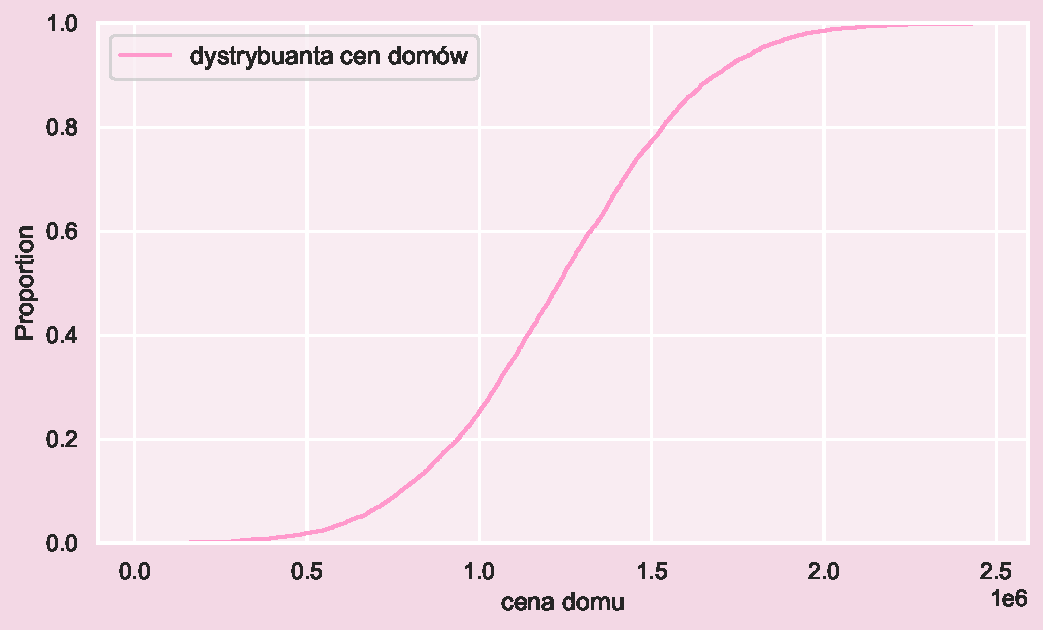
\includegraphics[scale=0.68]{images/price_dystr1.pdf}
		\caption{Dystrybuanta empiryczna cen domów}
		\label{denistyx}
	\end{center}
	\end{figure}
\noindent Z tego powodu tak samo jak przy zmiennej niezależnej wyznaczono parametry i dorysowano wykres dystrybuanty teoretycznej tym razem dla $\mu \approx 1232072 $ i $\sigma^2 \approx 124667119790 $. Kolejny raz otrzymano bardzo duże wartości, ale patrząc na to, że w tym raporcie pracuje się na cenach domów wartych miliony, takie rezultaty są jak najbardziej prawdopodobne.

    \begin{figure}[H]
	\begin{center}
		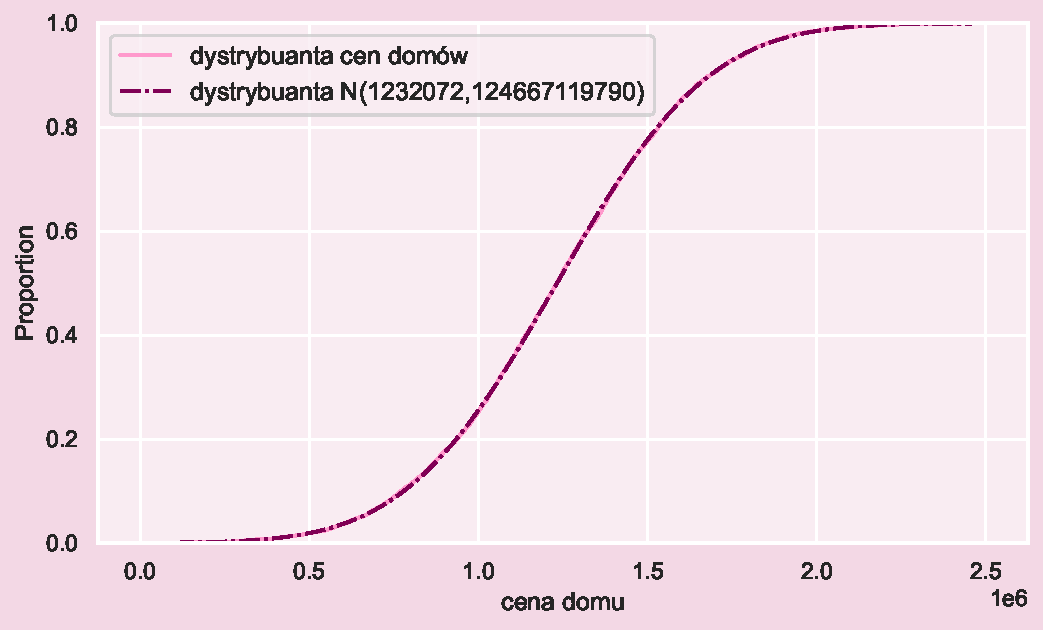
\includegraphics[scale=0.68]{images/price_dystr.pdf}
		\caption{Dystrybuanta empiryczna cen mieszkań i dystrybuanta teoretyczna rozkładu normalnego z parametrami $\mu \approx 1232072 $ i $\sigma^2 \approx 124667119790 $}
		\label{denistyx}
	\end{center}
	\end{figure}
\noindent Na ostatnim etapie wizualnej analizy zmiennej zależnej skupiono się na histogramie i informacjach, które można z niego wyciągnąć.
\begin{figure}[H]
	\begin{center}
		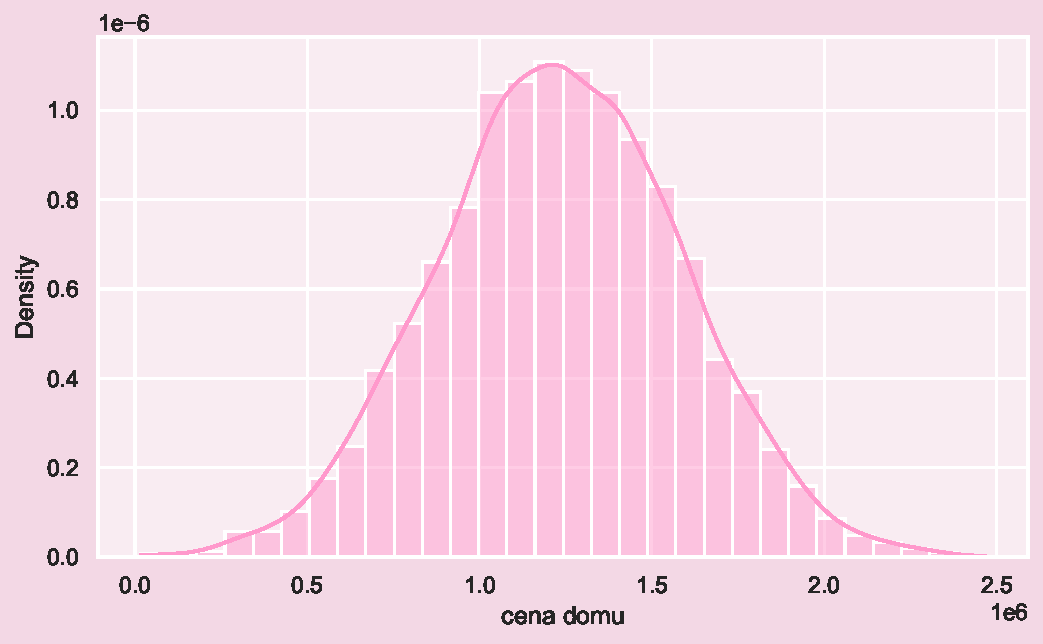
\includegraphics[scale=0.68]{images/price_hist.pdf}
		\caption{Histogram cen domów wraz z gęstością empiryczną}
		\label{denistyx}
	\end{center}
	\end{figure}
 \noindent Pokazuje on, że najbardziej popularną ceną jest $1.2$ miliona, a niewiele mniej domów zostaje sprzedane za kwotę z przedziału $1 - 1.5$ miliona. Symetryczność wykresu wskazuje, że ceny sa podobnie zróżnicowane powyżej i poniżej średniej. Najniższe słupki w okolicach $300$ tysięcy i powyżej $2.2$ miliona odpowiadają outlayersom z wykresu pudełkowego. Taki kształt wykresu od razu przysuwa na myśl rozkład normalny, a dorysowanie gęstości teoretycznej jedynie potwierdza ten fakt.

\begin{figure}[H]
	\begin{center}
		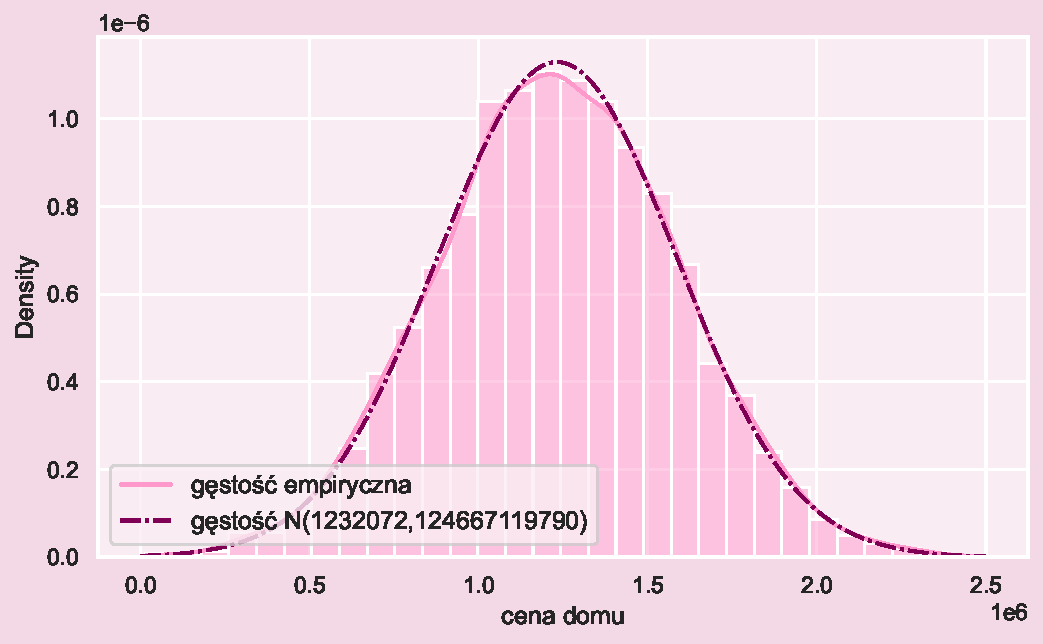
\includegraphics[scale=0.68]{images/price_hist_teor.pdf}
		\caption{Histogram cen domów wraz z gęstością empiryczną i teoretyczną}
		\label{denistyx}
	\end{center}
	\end{figure}
 

\subsubsection{Podstawowe miary}
Dla rozważanych danych obliczono także rózne miary i pogrupowano je w tabelach. 

\begin{table}[H]
\centering
\resizebox{\textwidth}{!}{%
\begin{tabular}{|cccccc|}
\hline
\rowcolor[HTML]{F66BB4} 
\multicolumn{6}{|c|}{\cellcolor[HTML]{F66BB4}\textbf{miary rozproszenia}}                                                                                                                                                                                                                                                                                                        \\ \hline
\rowcolor[HTML]{F2B7D6} 
\multicolumn{1}{|c|}{\cellcolor[HTML]{F2B7D6}\textbf{Q1}}   & \multicolumn{1}{c|}{\cellcolor[HTML]{F2B7D6}\textbf{Q3}}  & \multicolumn{1}{c|}{\cellcolor[HTML]{F2B7D6}\textbf{IQR}}      & \multicolumn{1}{c|}{\cellcolor[HTML]{F2B7D6}\textbf{wariancja}} & \multicolumn{1}{c|}{\cellcolor[HTML]{F2B7D6}\textbf{std}}  & \textbf{wsp. zmienności}                               \\ \hline
\rowcolor[HTML]{F5F5F5} 
\multicolumn{1}{|r|}{\cellcolor[HTML]{F5F5F5}997577.135049} & \multicolumn{1}{r|}{\cellcolor[HTML]{F5F5F5}1.471210e+06} & \multicolumn{1}{r|}{\cellcolor[HTML]{F5F5F5}473633.069163}     & \multicolumn{1}{r|}{\cellcolor[HTML]{F5F5F5}1.246671e+11}       & \multicolumn{1}{r|}{\cellcolor[HTML]{F5F5F5}353082.313053} & \multicolumn{1}{r|}{\cellcolor[HTML]{F5F5F5}28.660455} \\ \hline
\multicolumn{6}{|l|}{}                                                                                                                                                                                                                                                                                                                                                           \\ \hline
\rowcolor[HTML]{F66BB4} 
\multicolumn{6}{|c|}{\cellcolor[HTML]{F66BB4}\textbf{miary położenia}}                                                                                                                                                                                                                                                                                                           \\ \hline
\rowcolor[HTML]{F2B7D6} 
\multicolumn{2}{|c|}{\cellcolor[HTML]{F2B7D6}\textbf{śr. arytm.}}                                                       & \multicolumn{1}{c|}{\cellcolor[HTML]{F2B7D6}\textbf{śr.harm.}} & \multicolumn{1}{c|}{\cellcolor[HTML]{F2B7D6}\textbf{śr. geom.}} & \multicolumn{2}{c|}{\cellcolor[HTML]{F2B7D6}\textbf{mediana}}                                                       \\ \hline
\rowcolor[HTML]{FFFFFF} 
\multicolumn{2}{|r|}{\cellcolor[HTML]{FFFFFF}1.232073e+06}                                                              & \multicolumn{1}{r|}{\cellcolor[HTML]{FFFFFF}1.081459e+06}      & \multicolumn{1}{r|}{\cellcolor[HTML]{FFFFFF}1.173387e+06}       & \multicolumn{2}{c|}{\cellcolor[HTML]{FFFFFF}1.232669e+06}                                                           \\ \hline
\rowcolor[HTML]{FFFFFF} 
\multicolumn{6}{|l|}{\cellcolor[HTML]{FFFFFF}}                                                                                                                                                                                                                                                                                                                                   \\ \hline
\rowcolor[HTML]{F66BB4} 
\multicolumn{6}{|c|}{\cellcolor[HTML]{F66BB4}{\color[HTML]{000000} \textbf{miary skośności i spłaszczenia}}}                                                                                                                                                                                                                                                                     \\ \hline
\rowcolor[HTML]{F2B7D6} 
\multicolumn{3}{|c|}{\cellcolor[HTML]{F2B7D6}\textbf{wsp. skośności}}                                                                                                                    & \multicolumn{3}{c|}{\cellcolor[HTML]{F2B7D6}\textbf{kurtoza}}                                                                                                                         \\ \hline
\rowcolor[HTML]{FFFFFF} 
\multicolumn{3}{|c|}{\cellcolor[HTML]{FFFFFF}-0.002717}                                                                                                                                  & \multicolumn{3}{c|}{\cellcolor[HTML]{FFFFFF}0.056063}                                                                                                                                 \\ \hline
\end{tabular}%
}
\caption{Miary dla cen domów}
\label{miary_price}
\end{table}

\noindent Tym razem również wartość kurtozy $-0.056063$ stanowi kolejne potwierdzenie, że prawidłowo zidentyfikowano rozkład omawianej zmiennej.

\subsubsection{Wnioski}
W powyższym podrozdziale rozłożono na czynniki pierwsze zmienną zależną, co zaowocowało znalezieniem jej rozkładu i poznaniem chrakterystyki występujących wartości. Dodatkowo nie znaleziono istotnie odstających wartości. Wszystko to sprawia, że przeanalizowane dane doskonale nadają się do zbudowania modelu regresji liniowej.
\section{Analiza zależności liniowej pomiędzy zmienną objaśniającą a zmienną objaśnianą}

\subsection{Prezentacja danych}

    \begin{figure}[H]
	\begin{center}
		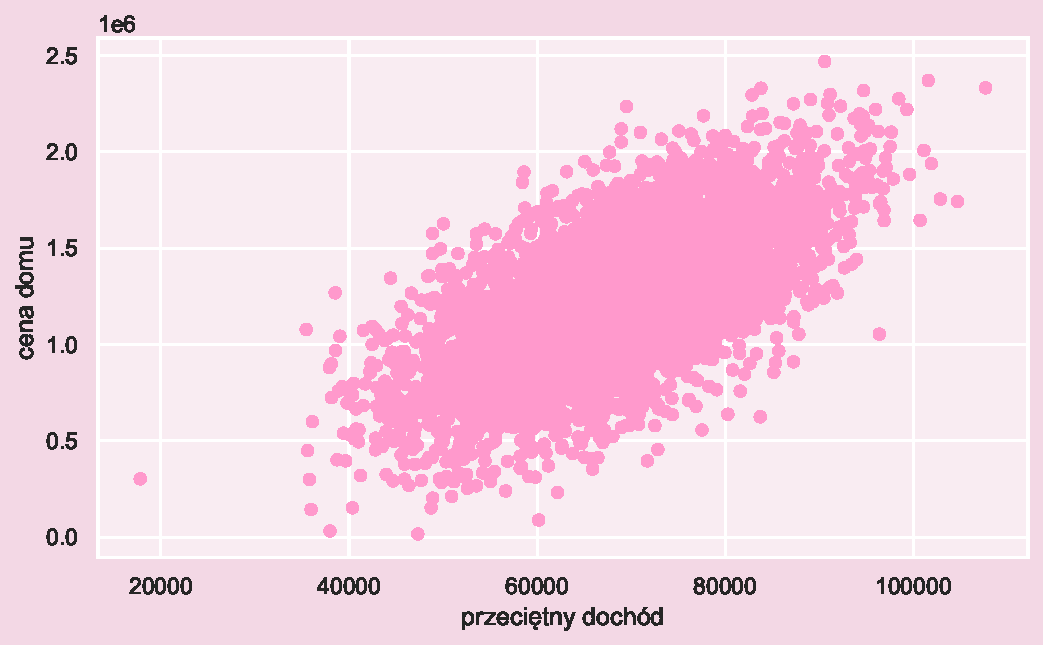
\includegraphics[scale=0.68]{images/scatter1.pdf}
		\caption{Wysokość ceny domu w zależności od przeciętnego dochodu w jego okolicy}
		\label{scatterxy}
	\end{center}
	\end{figure}

Na wykresie rozproszenia danych (Rysunek \ref{scatterxy}) widać wyraźną zależność liniową. Ponieważ obserwacje układają się wzdłuż jednej prostej, ale nie są wokół niej ściśle skumulowane, możemy wyciągnąć wniosek, że powyższa korelacja nie jest bardzo silna. Potwierdza to współczynnik Pearsona, który wynosi $0.64$.
 
\subsection{Estymacja współczynników w klasycznym modelu regresji liniowej}
Podczas analizy danych wykorzystano klasyczny model regresji liniowej. Ma on następujące założenia:
\begin{itemize}
    \item ${\mathbb{E}} \varepsilon_i = 0 \quad \forall i = 1,2,...,n$
    \item $Var \varepsilon_i = \sigma^2 \quad \forall i = 1,2,...,n$
    \item $\varepsilon_1, \varepsilon_2,...,\varepsilon_n$ - niezależne zmienne losowe
    \item $\varepsilon_i \sim \mathcal{N} (\mu,\sigma^2) \quad \forall i = 1,2,...,n $
\end{itemize} 
Proces estymacji współczynników można przeprowadzić na dwa sposoby. Estymacja punktowa korzysta z metody najmniejszych kwadratów lub metody największej wiarygodności. Znając teorię, można wyprowadzić wzory na estymatory współczynników. Natomiast estymacja przedziałowa zakłada skonstruowanie przedziałów ufności dla $B_0$ i $B_1$. Korzystając z tego sposobu, można stwierdzić, że na wybranym pozomie istotności $\alpha$, współczynniki $B_0,B_1$ mieszczą się w uzyskanym przedziale z prawdopodobieństwem $1-\alpha$.

\subsubsection{Estymacja punktowa}
\noindent Współczynniki prostej regresji wyznaczono z wykorzystaniem metody najmniejszych kwadratów. Estymatory wynoszą 
$$\hat{B_1} = \cfrac{\sum_i^n x_i {\left( y_i - \overline{y} \right) }^2}{\sum_i^n {\left( x_i - \overline{x} \right)}^2 } = 21.195$$
$$\hat{B_0} = \overline{y} - \hat{B_1} \overline{x} = -221579.478.$$

    \begin{figure}[H]
	\begin{center}
		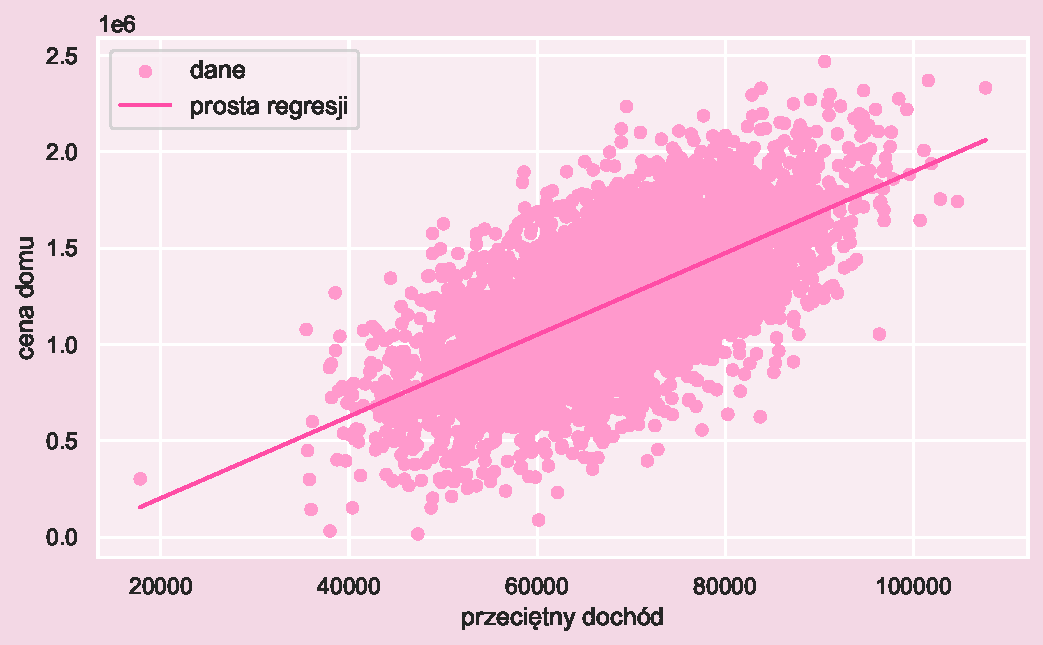
\includegraphics[scale=0.68]{images/regresja.pdf}
		\caption{Dopasowanie prostej regresji o współczynnikach $\hat{B_0} = 21.195$, $\hat{B_1} = -221579.478$}
		\label{denistyx}
	\end{center}
	\end{figure}

\subsubsection{Estymacja przedziałowa}
Do obliczeń wykorzystano poziom istotności $\alpha = 0.05$, zatem współczynniki $B_0,B_1$ znajdują się w poniższych przedziałach z prawdopodobieństwem $95\%$. Dla $B_0$ wykorzystano wzór
$$\left[\hat{B_0} - t_{1-\frac{\alpha}{2},n-2} \cdot S \sqrt{ \cfrac{1}{n} +\cfrac{{\overline{x}}^2}{\sum_i^n {\left( x_i - \overline{x} \right) }^2}}, \quad
\hat{B_0}+ t_{1-\frac{\alpha}{2},n-2} \cdot S \sqrt{ \cfrac{1}{n} +\cfrac{{\overline{x}}^2}{\sum_i^n {\left( x_i - \overline{x} \right) }^2}} \right] =$$

$$\left[ -221579.6587, -221579.2976 \right] .$$ \\


Podobnie dla współczynnika $B_1$:
$$\left[\hat{B_1} - t_{1-\frac{\alpha}{2},n-2} \cdot \cfrac{S}{\sqrt{\sum_i^n {\left( x_i - \overline{x} \right) }^2}}, 
\quad
\hat{B_1}+ t_{1-\frac{\alpha}{2},n-2} \cdot \cfrac{S}{\sqrt{\sum_i^n {\left( x_i - \overline{x} \right) }^2}} \right] =$$

$$\left[ 20.4893, 21.9016\right].$$ \\ 
 
\subsection{Jakość dopasowania w modelu regresji liniowej}
Jakość dopasowania prostej regresji można sprawdzić za pomocą współczynnika determinacji $\phi = \cfrac{SSR}{SST} = \cfrac{SST-SSE}{SST}$, gdzie:
\begin{itemize}
    \item SSE = $\sum_i^n {\left( y_i - \hat{y_i} \right)}^2$
    \item SSR = $\sum_i^n {\left( \hat{y_i} - \overline{y} \right)}^2$
    \item SST = SSE + SSR.
\end{itemize}
Dla analizowanych danych współczynnik ten wynosi $0.409$. Oznacza to, że $40.9\%$ zmiennych objaśnianych udało się opisać za pomocą zmiennych objaśniających.
Rozpisujac wzory na powyższe wskaźniki, otrzymamy kwadrat współczynnika korelacji Pearsona. Istotnie, korzystając z wcześniejszych obliczeń, ${\left( 0.64 \right)}^2 = 0.409$.

\subsection{Predykcja oraz przedziały ufności dla danych testowych}
Predykcja oraz ocena jej efektywności przebiega według poniższego algorytmu.
\begin{enumerate}
    \item Podział danych na zbiór treningowy i zbiór testowy.
    \item Wyznaczenie współczynników $\hat{B_0}$ i $\hat{B_1}$ na podstawie zbioru treningowego.
    \item Wyznaczenie prostej regresji na zbiorze treningowym. Wyliczenie błędów i znalezienie ich rozkładu.
    \item Wyznaczenie predykowanych wartości na zbiorze testowym, uwzględniając błędy jako zmienne z poznanego rozkładu.
    \item Wyznaczenie przedziałów ufności dla zbioru testowego na poziomie istotności $\alpha$.
    \item Zliczenie jaka część wartości predykowanych oraz jaka część danych rzeczywistych ze zbioru testowego znalazła się w wyliczonym przedziale ufności. Uzyskane ułamki powinny w przybliżeniu równać się $1-\alpha$.
\end{enumerate}


    \begin{figure}[H]
	\begin{center}
		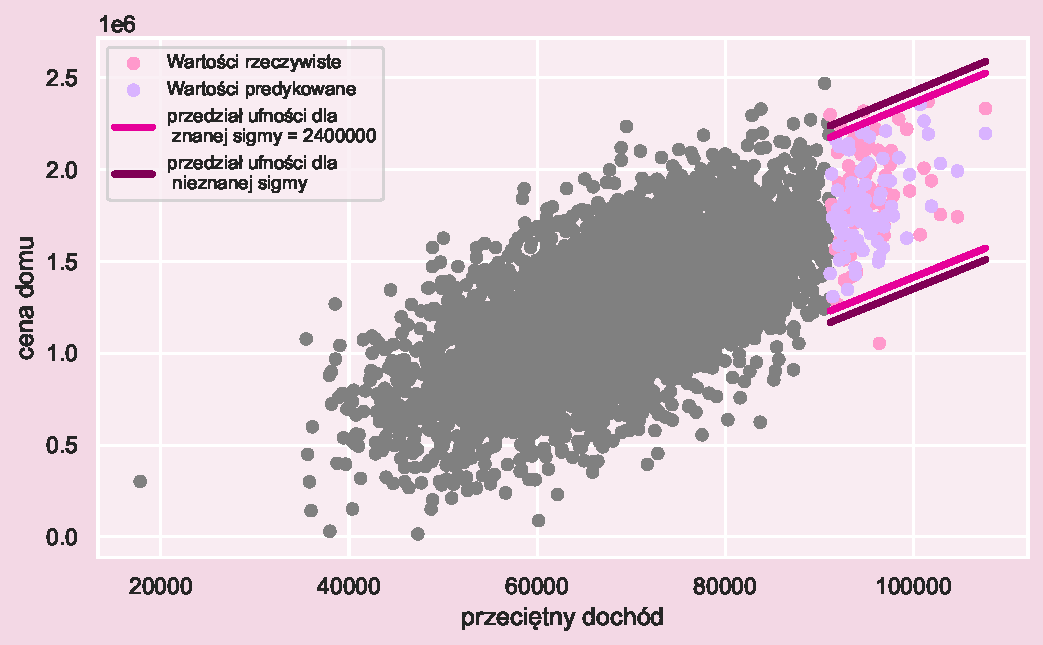
\includegraphics[scale=0.68]{images/predykcja.pdf}
		\caption{Predykcja oraz przedziały ufności dla danych testowych}
		\label{prediction1}
	\end{center}
	\end{figure}
 
    \begin{figure}[H]
	\begin{center}
		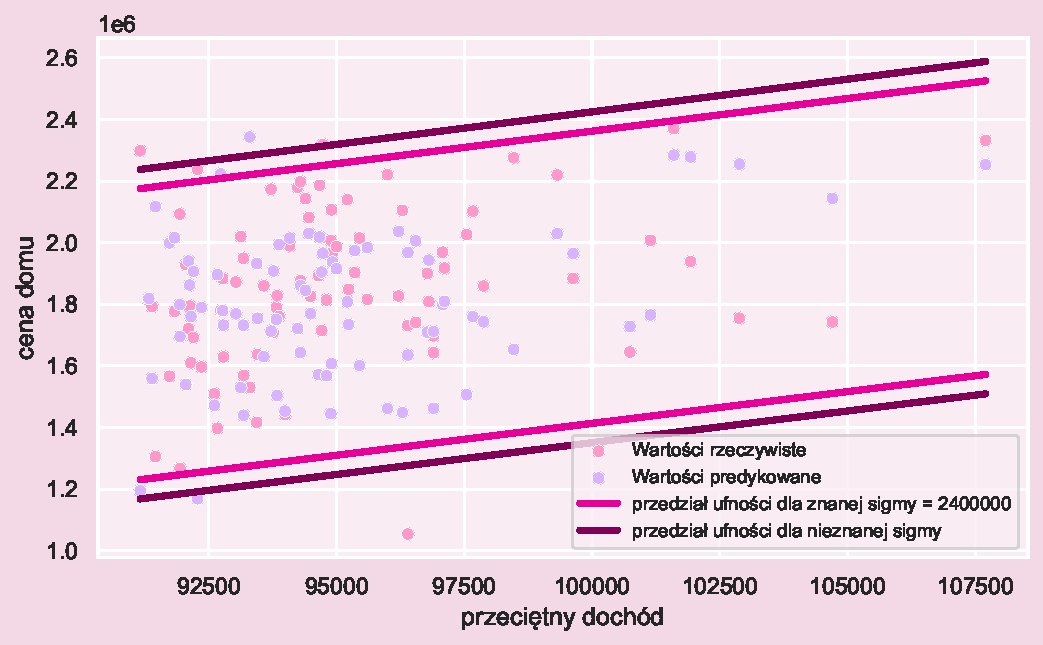
\includegraphics[scale=0.68]{images/predykcja_zoom.pdf}
		\caption{Predykcja oraz przedziały ufności dla danych testowych}
		\label{prediction2}
	\end{center}
	\end{figure}

\noindent Zgodnie z algorytmem, analizowane dane zostały podzielone na dwie grupy. Zbiór testowy składa się z 80 obserwacji o największym przeciętnym dochodzie. Współczynniki regresji liniowej wyliczone dla zbioru treningowego wynoszą $\hat{B_0}=-202938.6469$ i $\hat{B_1}=20.905821$, a błędy pochodzą z rozkładu $N(\mu=0,\sigma=271377)$. Przedziały ufności zostały skonstruowane ze wzoru 
$$\left[\hat{y}\left( x_0 \right) - t_{1-\frac{\alpha}{2},n-2} \cdot S \sqrt{ 1+\cfrac{1}{n} + \cfrac{ {\left( x_0 - \overline{x} \right) }^2}{\sum_i {\left( x_i - \overline{x} \right) }^2}}, 
\quad
\hat{y}\left( x_0 \right) + t_{1-\frac{\alpha}{2},n-2} \cdot S \sqrt{ 1+\cfrac{1}{n} + \cfrac{ {\left( x_0 - \overline{x} \right) }^2}{\sum_i {\left( x_i - \overline{x} \right) }^2}}\right]$$
W obliczeniach wykorzystano poziom istotności $\alpha = 0.05$ oraz nieobciążony estymator odchylenia standardowego $S=\sqrt{\frac{1}{n-2} \sum_i \left( Y_i - \hat{Y_i} \right)}$. Dla porównania, na wykresach \ref{prediction1} i \ref{prediction2} przedstawiono również przedział ufności wyliczony sposobem dla znanej sigmy, równej $240000$. Fakt, że owy przedział jest węższy od nominalnego sugeruje, że prawdziwa wartość $\sigma$ jest większa niż przyjęto w tej metodzie. \\


\subsection{Ocena jakości dopasowania do danych testowych}
Dla poziomu istotności $\alpha = 0.05$ procenty danych predykowanych i danych rzeczywistych zawartych w przedziale ufności wynosiły odpowiednio
$96.25\%$ i $95\%$. Uzyskane liczby w przybliżeniu równają się $1-\alpha$. Oznacza to, że sposób predykowania danych został zaimplementowany poprawnie. \\

\noindent Otrzymane przedziały ufności można zastosować także dla wszystkich cen domów.
 
 \begin{figure}[H]
	\begin{center}
		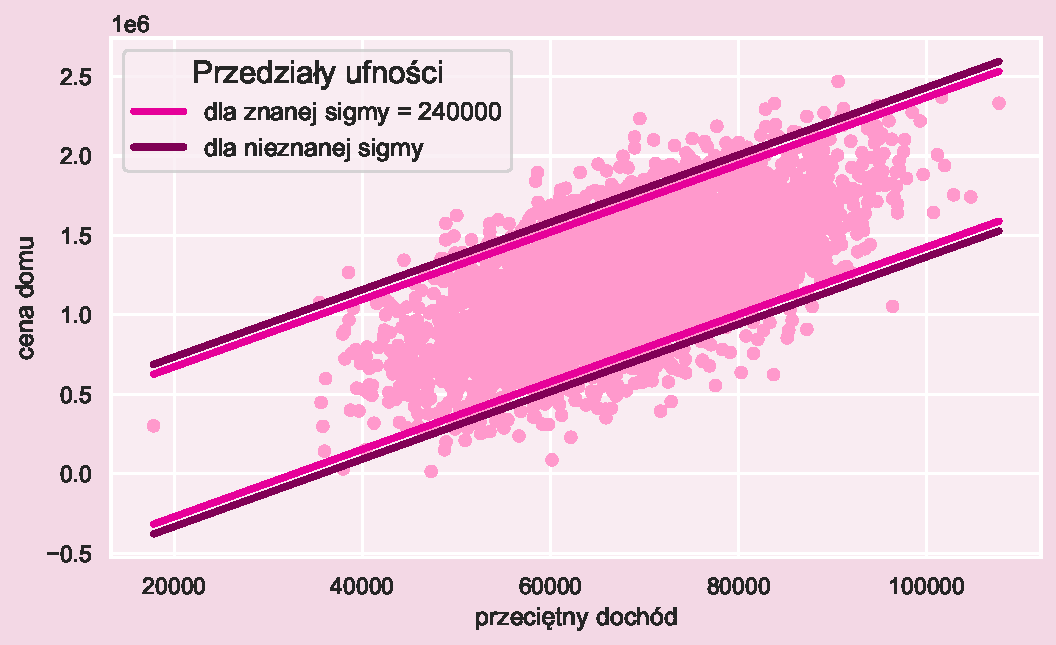
\includegraphics[scale=0.68]{images/przedzialy_ufnosci.pdf}
		\caption{Przedziały ufności dla znanej i nieznanej wariancji}
		\label{denistyx}
	\end{center}
	\end{figure}

 \noindent Dla empirycznie wyliczonego przedziału ufności (nieznana sigma) $94.82\%$ obserwacji znajduje się między prostymi. 

\subsection{Wnioski}
Wykonanie powyższych analiz doprowadziło do wyznaczenia estymatorów współczynników $B_0$ i $B_1$ oraz ich przedziałów ufności na poziomie istotności $\alpha = 0.05$. Oceniono także jakość dopasowania w modelu regresji liniowej za pomocą współczynnika determinacji, który wyniósł $0.49$. Otrzymane rezultaty zaprezentowano na wykresie. Na koniec poprawnie zaimplementowano sposób predykcji danych i sprawdzono jego efektywność.
\section{Analiza residuów}

\subsection{Sprawdzenie założeń}
Chcąc stwierdzic, czy poprawnie wyznaczono współczynniki $\hat{B_0}$ i $\hat{B_1}$ konieczne jest wykonanie analizy residuów, czyli wartości resztkowych w modelu regresji liniowej. Muszą one spełniać następujące warunki:
\begin{itemize}
    \item ${\mathbb{E}} \varepsilon_i = 0 \quad \forall i = 1,2,...,n$
    \item $Var \varepsilon_i = \sigma^2 \quad \forall i = 1,2,...,n$
    \item $\varepsilon_1, \varepsilon_2,...,\varepsilon_n$ - niezależne zmienne losowe
    \item $\varepsilon_i \sim \mathcal{N} (\mu,\sigma^2) \quad \forall i = 1,2,...,n $
\end{itemize} 
By móc powiedzieć coś więcej na temat wartości oczekiwanej i wariancji residuów, sporządzono wykres punktowy przedstawiający wszystkie residua.
\begin{figure}[H]
	\begin{center}
		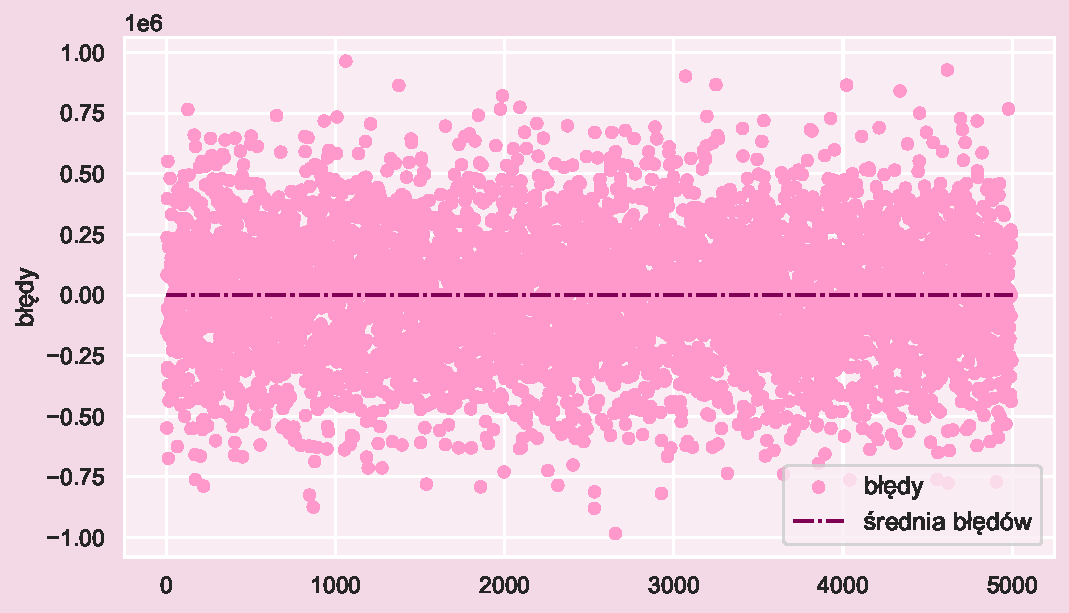
\includegraphics[scale=0.68]{images/resi_scatter.pdf}
		\caption{Wykres punktowy wartości resztkowych}
		\label{denistyx}
	\end{center}
    \end{figure}
\noindent Juz na pierwszy rzut oka widać, że błędy rozkładają się równomiernie po obu stronach osi poziomej. Dodatkowo potwierdza to ich średnia, którą również naniesiono na wykres. Jej wartość policzona przy pomocy funkcji wbudowanej w Pythonie to $1.19791e-9$. Już na tym etapie można także stwierdzić, że residua mają stałą wariancję (według wbudowanej funkcji jest to $73645940735.18942$, ponieważ tworzą w przybliżeniu pas jednej grubości. \\\\
Następnie sprawdzono, czy rozważane dane są niezależnymi zmiennymi losowymi. W tym celu posłużono się dwiema funkcjami: 
\begin{itemize}
    \item empirycznej autokowariancji 
 \begin{align*}
        \hat{\gamma}(h) = \frac{1}{n} \sum\limits_{i=1}^{n-|h|} (e_{i+|h|}-\bar{e})(e_i-\bar{e}) \quad -n<h<n,\quad h \in Z,
    \end{align*}
    \item empirycznej autokorelacji
 \begin{align*}
        \hat{g}(h) = \frac{\hat{\gamma}(h)}{\hat{\gamma}(0)}. 
    \end{align*}
\end{itemize}
Najpierw policzono funkcję empirycznej autokowariancji dla wszystkich możliwych wartości $h$, a następnie wyznaczono empiryczną autokorelację i to ją przedstawiono na wykresie \ref{acf}.
    \begin{figure}[H]
	\begin{center}
		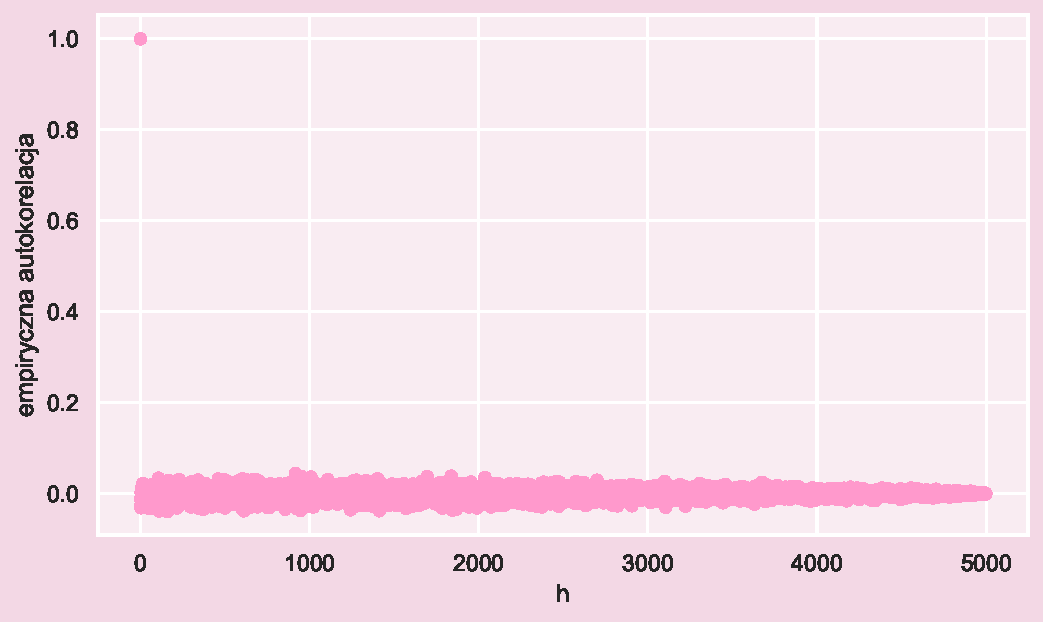
\includegraphics[scale=0.68]{images/acf.pdf}
		\caption{Wykres funkcji empirycznej autokorelacji w zależności od $h$}
		\label{acf}
	\end{center}
    \end{figure}
\noindent Funkcja dla $h=1$ wynosi $1$ a poza tym wszędzie jest bliska zeru. Taka postac funkcji autokorelacji empirycznej dowodzi, że badane residua są zmiennymi niezależnymi.\\

Ostatnim założeniem jakie należy udowodnić jest pochodzenie wartości resztkowych z rozkładu normalnego o zerowej średniej i stałej wariancji. Jednym ze sposobów, by to osiągnąć, jest narysowanie histogramu i próba dopasowania gęstości rozkładu normalnego o odpowiednich parametrach. 
    \begin{figure}[H]
	\begin{center}
		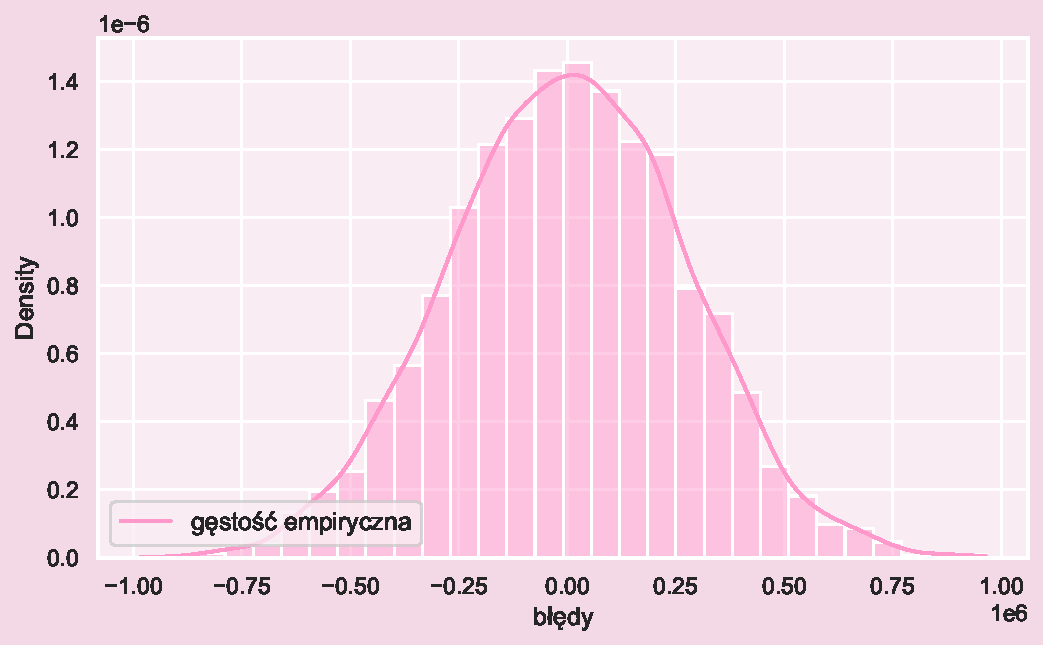
\includegraphics[scale=0.68]{images/resi_hist.pdf}
		\caption{Histogram wartości resztkowych}
		\label{denistyx}
	\end{center}
    \end{figure}
\noindent Ponieważ histogram kształtem bardzo przypomina rozkład normalny o średniej zero, najrozsądniejszym jest dorysowanie gęstości rozkładu normalnego o parametrach równych wariancji i średniej wyznaczonych na początku tego podrozdziału.
    \begin{figure}[H]
	\begin{center}
		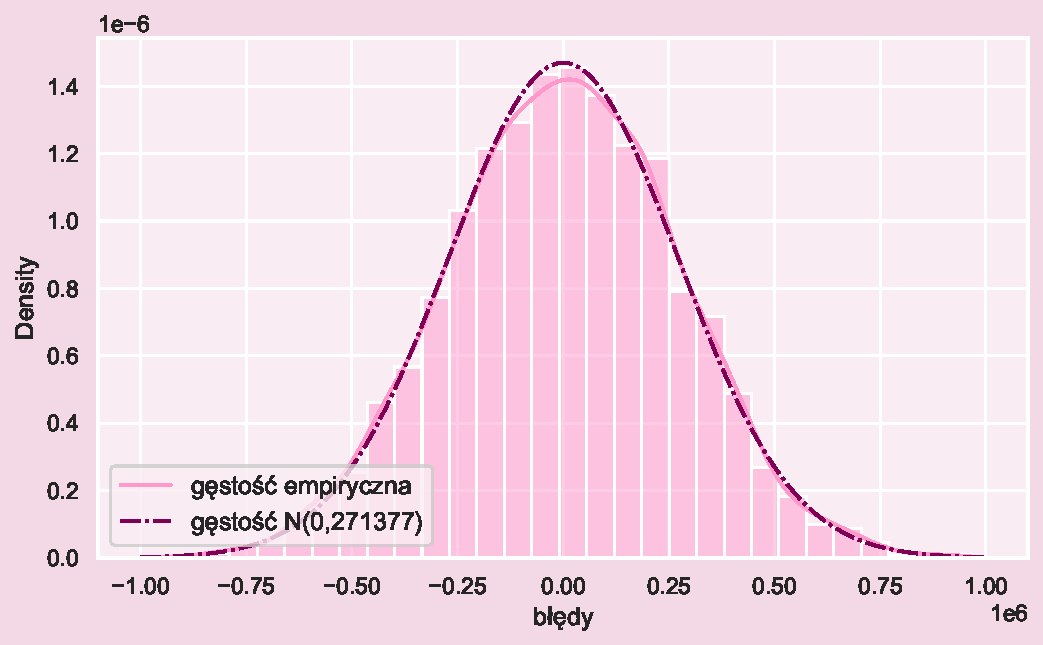
\includegraphics[scale=0.68]{images/resi_hist_teor.pdf}
		\caption{Histogram wartości resztkowych wraz z gęstością empiryczną i teoretyczną z rozkładu  $\mathcal{N}$$(0,73645940735)$ }
		\label{resi_hist_teor}
	\end{center}
    \end{figure}
\noindent Na wykresie \ref{resi_hist_teor}. obie gęstości pokrywają się, a ponieważ gęstość jednoznacznie identyfikuje rozkład, jest to dowód na to, że residua pochodzą z rozkładu normalnego o średniej zero i stałej wariancji. Dodatkowo wykonano wykres kwantylowy i jako rozkład teoretyczny przyjęto $\mathcal{N}$$(0,73645940735)$. Nachylenie linii kwantylowej do osi poziomej pod kątem $45^\circ$ ostatecznie potwierdza wysnuty wniosek.


\subsection{Wnioski}
W podrozdziale tym wzięto pod lupę residua i dokładnie przeanalizowano je pod kątem spełniania założeń niezbędnych w regresji liniowej. Ponieważ w odniesieniu do każdego z nich otrzymano satysfakcjonujące rezultaty, można stwierdzić, że poprawnie zbudowano model regresji liniowej.
\section{Podsumowanie}
Podsumowując raport można stwierdzić, że zrealizowano wszystkie postawione na początku cele. Skrupulatnie przeanalizowano dane i sprawdzono poprawność założeń. Zdołano zidentyfikować rozkłady z jakich pochodziły zmienne i poprawnie wyznaczyć współczynniki w modelu regresji linowej. Praca z danymi oparta na statystyce i programowaniu zaowocowała w tym przypadku dobraniem właściwego modelu do danych i wykonaniem predykcji dla cen domów w zależności od średnich zarobków w jego okolicy. 
\end{document}